\begin{figure}[!htbp]
\centering
\renewcommand{\arraystretch}{0.8}
\begin{tabular}{|c c c c c|}
	
\hline

(a) & (b) & (c) & (d) & (e) \\

\hline
{} & {} & {} & {} & {} \\

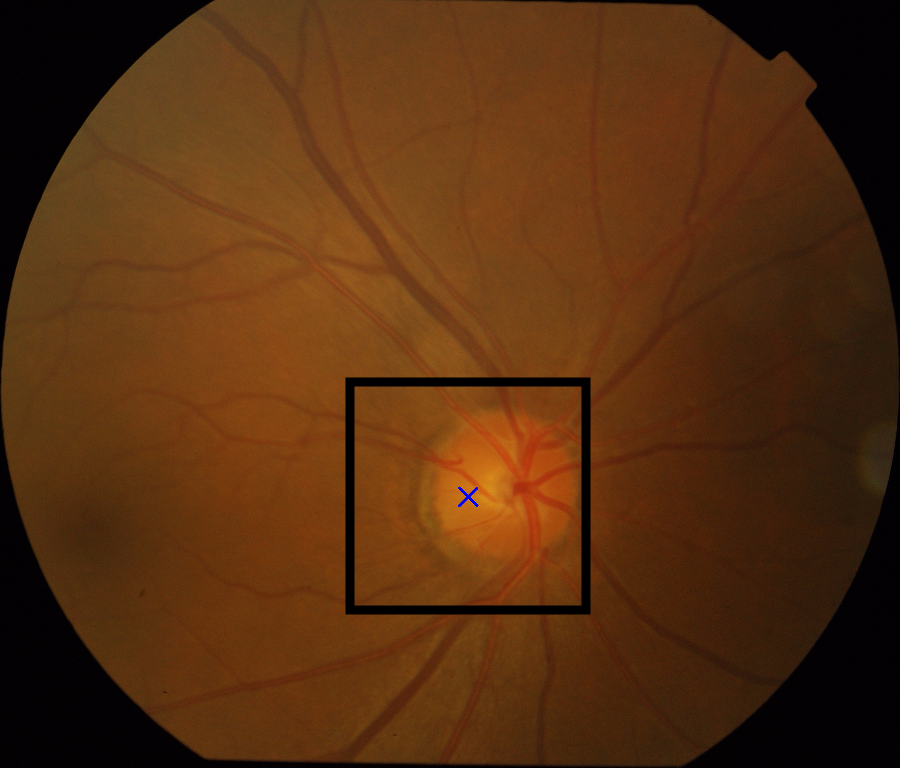
\includegraphics[width=3.5cm]{Images/Results/Results/drishti47/od_detect_frame.png} &
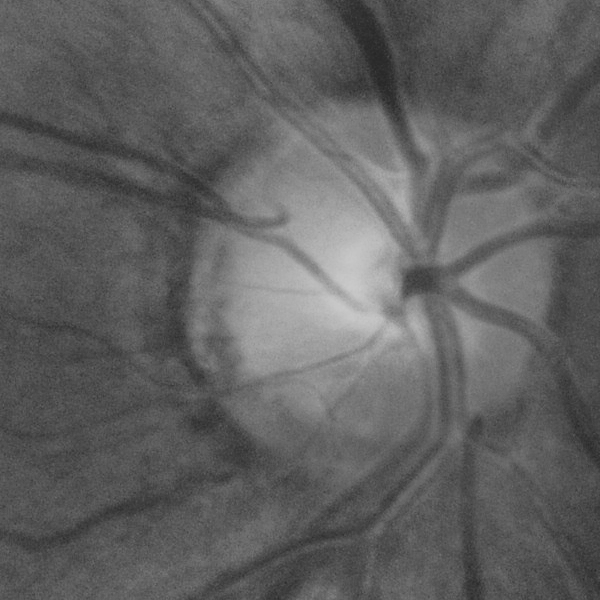
\includegraphics[width=3cm]{Images/Results/Results/drishti47/0_crop.png} &
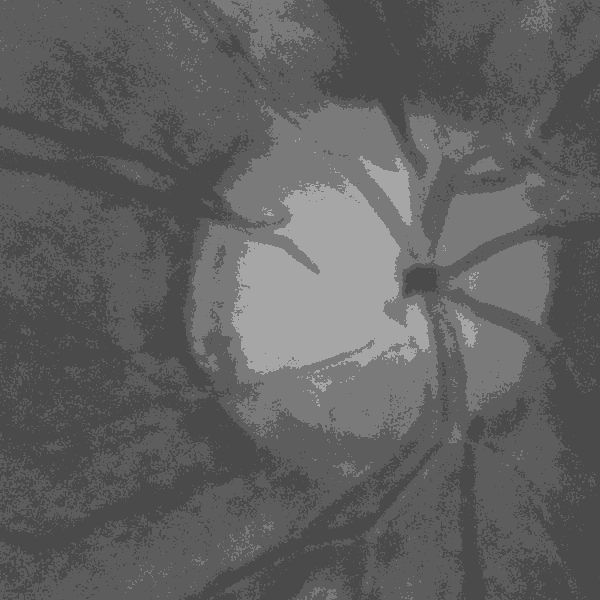
\includegraphics[width=3.0cm]{Images/Results/Results/drishti47/1_kmeans.png} &
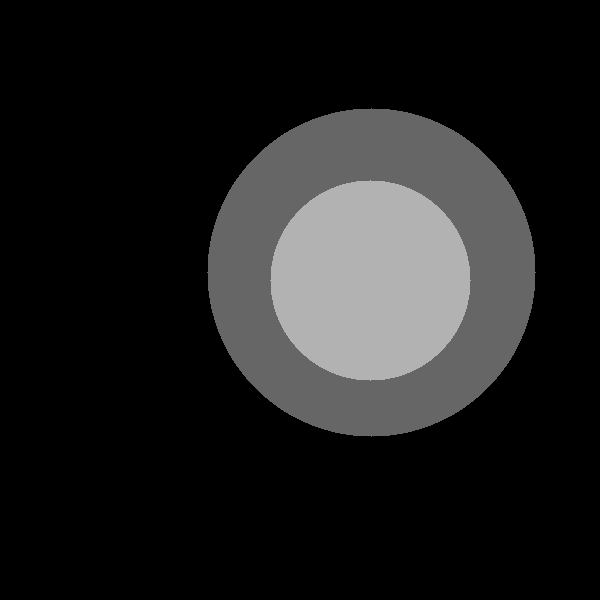
\includegraphics[width=3cm]{Images/Results/Results/drishti47/overlay.png} &
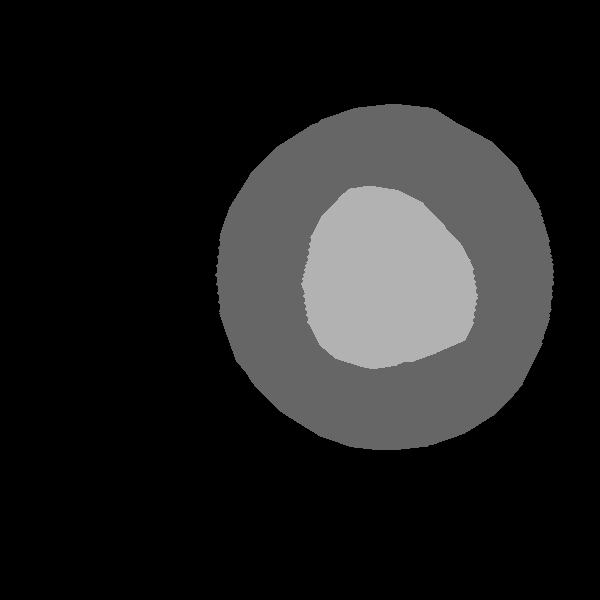
\includegraphics[width=3cm]{Images/Results/Results/drishti47/overlay_gt.png} \\

{} & {} & {} & CDR = 0.42 & CDR = 0.36 \\
{} & {} & {} & $\updownarrow$ & $\updownarrow$ \\
{} & {} & {} & Healthy & Healthy \\

\hline

{} & {} & {} & {} & {} \\

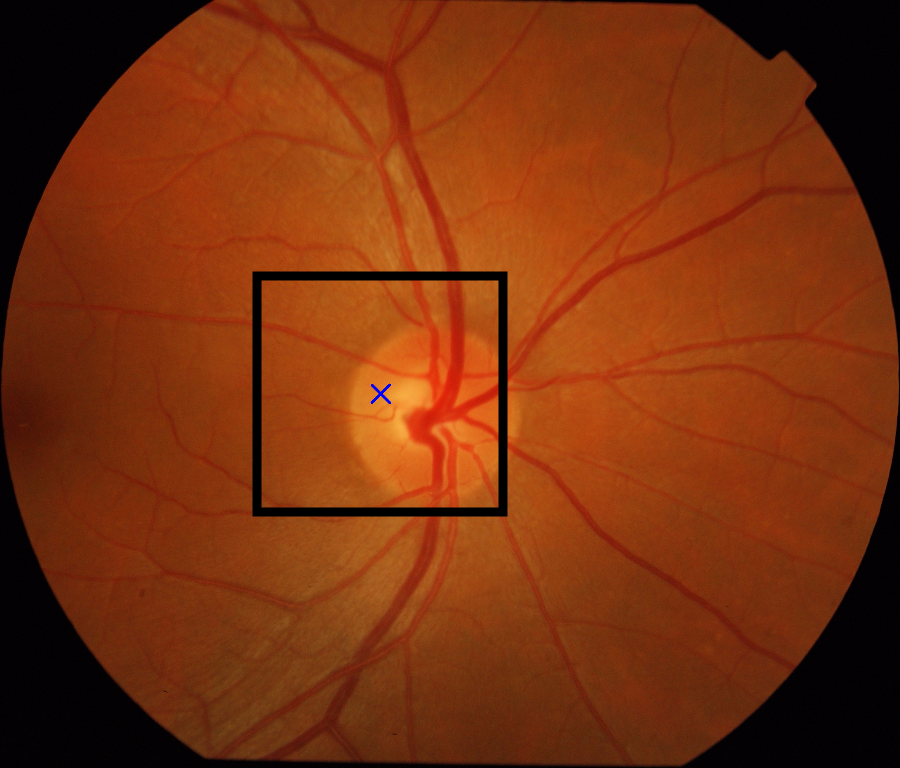
\includegraphics[width=3.5cm]{Images/Results/Results/drishti42/od_detect_frame.png} &
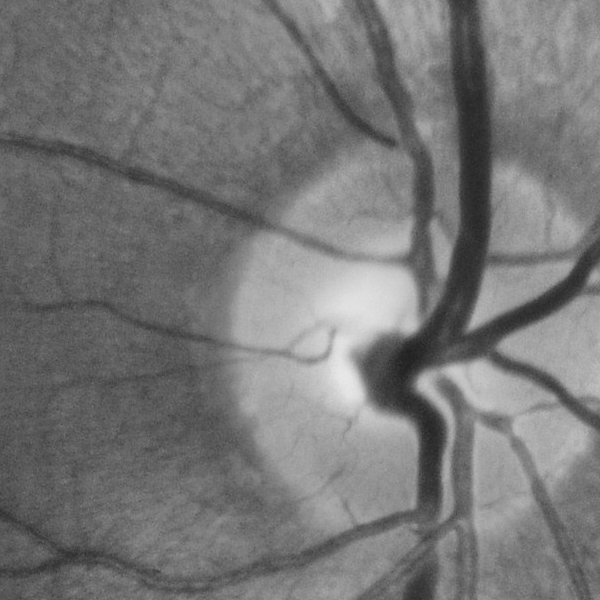
\includegraphics[width=3cm]{Images/Results/Results/drishti42/0_crop.png} & 
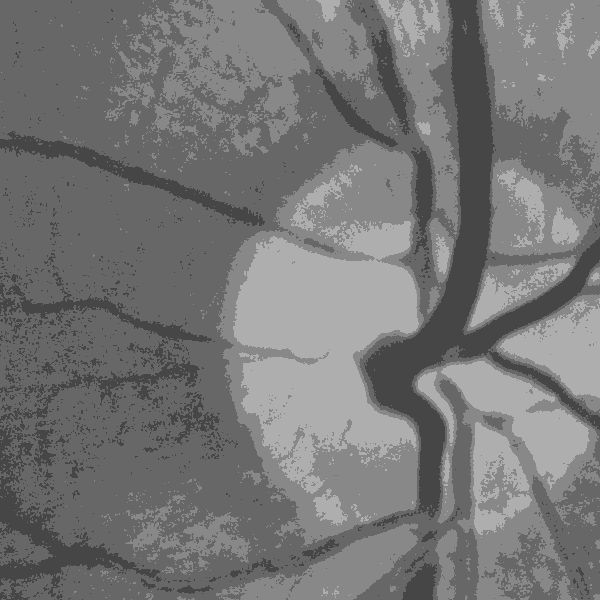
\includegraphics[width=3.0cm]{Images/Results/Results/drishti42/1_kmeans.png} &
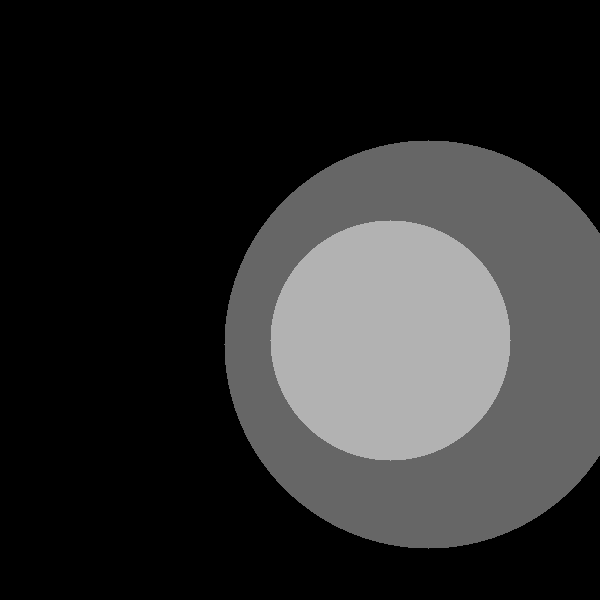
\includegraphics[width=3cm]{Images/Results/Results/drishti42/overlay.png} &
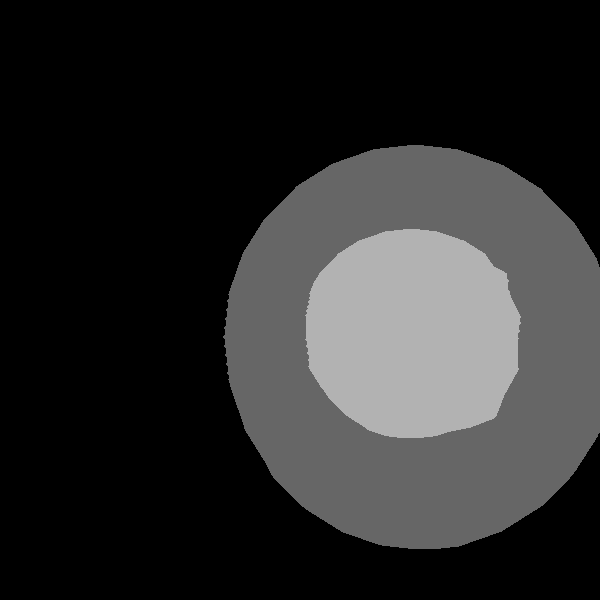
\includegraphics[width=3cm]{Images/Results/Results/drishti42/overlay_gt.png} \\

{} & {} & {} & CDR = 0.40 & CDR = 0.34 \\
{} & {} & {} & $\updownarrow$ & $\updownarrow$ \\
{} & {} & {} & Healthy & Healthy \\

\hline

{} & {} & {} & {} & {} \\

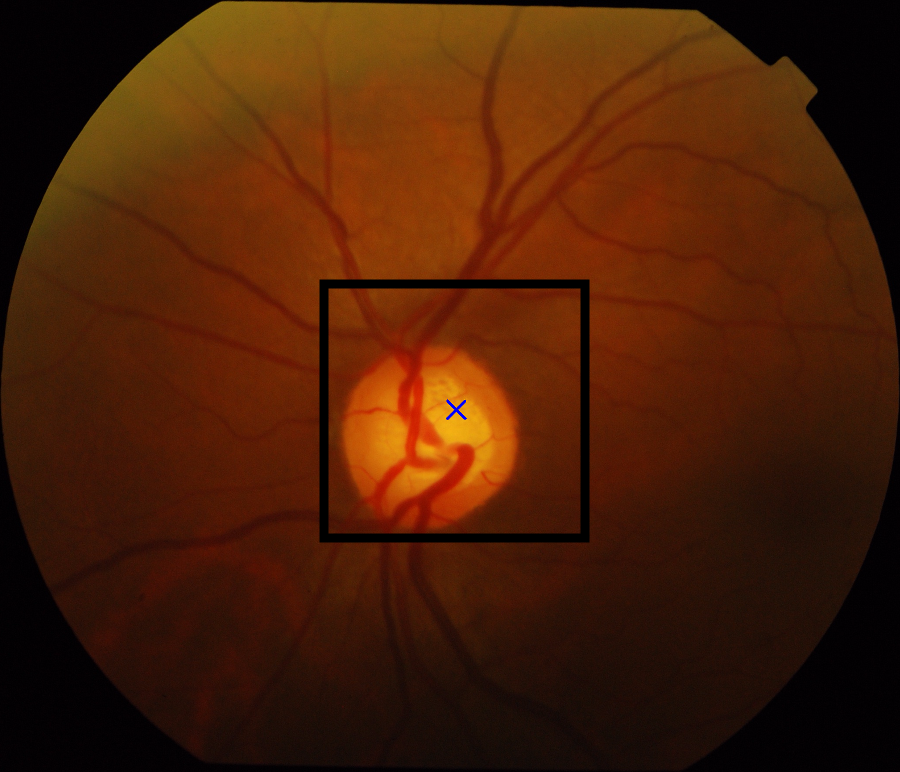
\includegraphics[width=3.5cm]{Images/Results/Results/drishti36/od_detect_frame.png} &
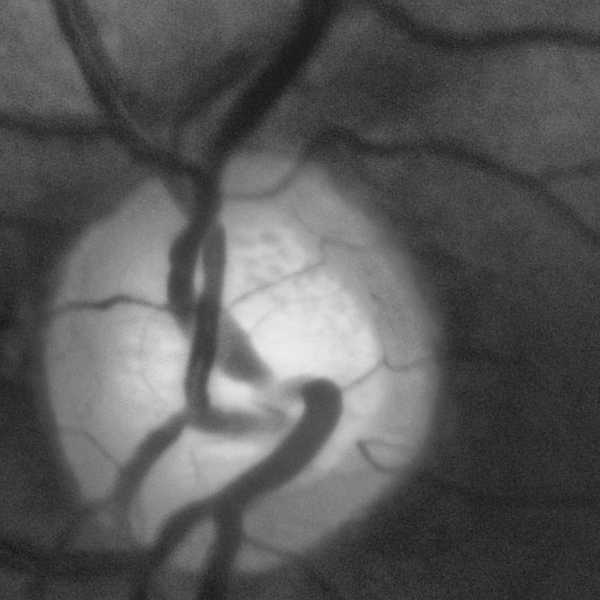
\includegraphics[width=3cm]{Images/Results/Results/drishti36/0_crop.png} &
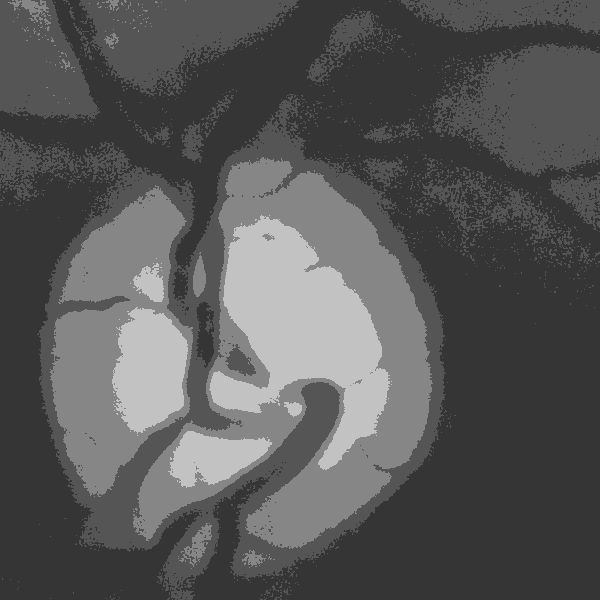
\includegraphics[width=3.0cm]{Images/Results/Results/drishti36/1_kmeans.png} &
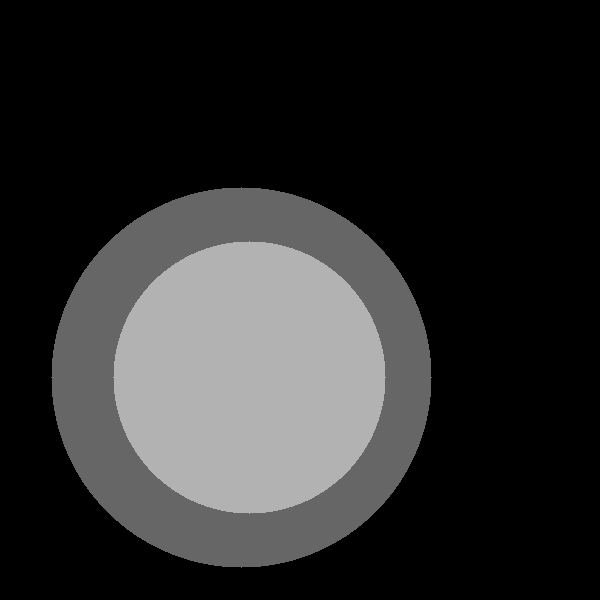
\includegraphics[width=3cm]{Images/Results/Results/drishti36/overlay.png} &
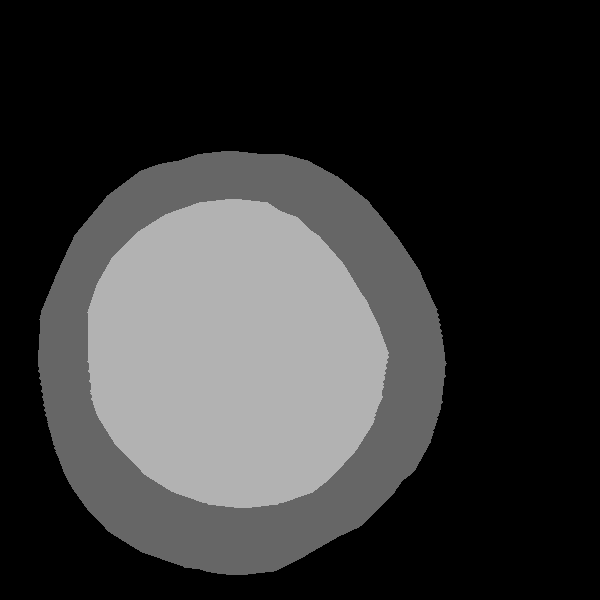
\includegraphics[width=3cm]{Images/Results/Results/drishti36/overlay_gt.png} \\

{} & {} & {} & CDR = 0.68 & CDR = 0.70 \\
{} & {} & {} & $\updownarrow$ & $\updownarrow$ \\
{} & {} & {} & Glaucomatous & Glaucomatous \\

\hline

{} & {} & {} & {} & {} \\

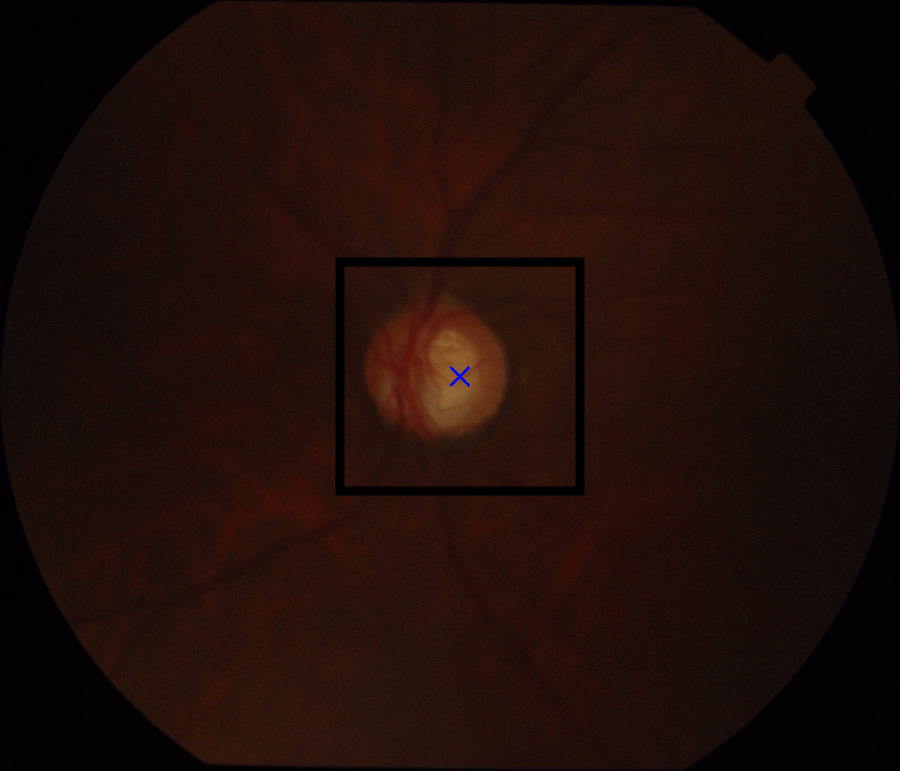
\includegraphics[width=3.5cm]{Images/Results/Results/drishti02/od_detect_frame.png} &
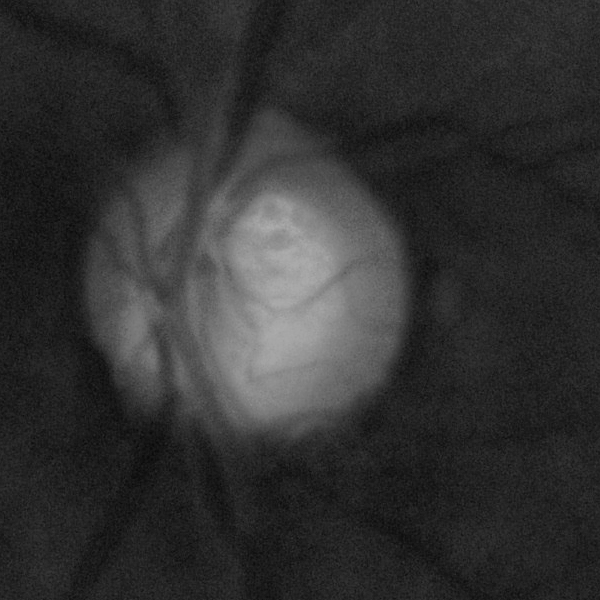
\includegraphics[width=3cm]{Images/Results/Results/drishti02/0_crop.png} &
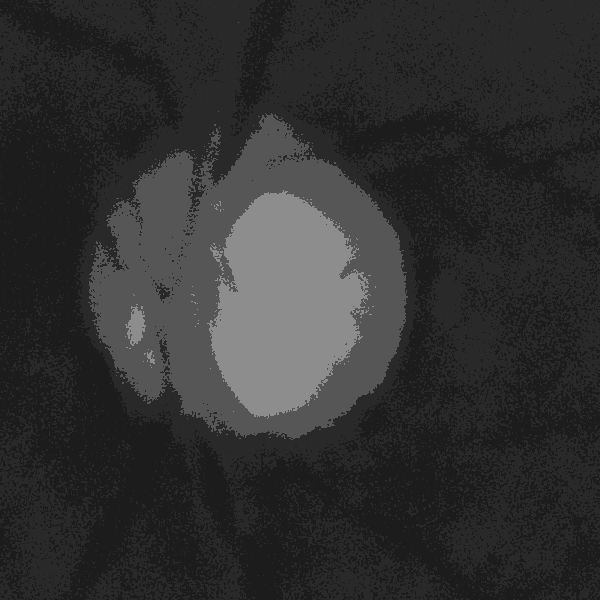
\includegraphics[width=3.0cm]{Images/Results/Results/drishti02/1_kmeans.png} & 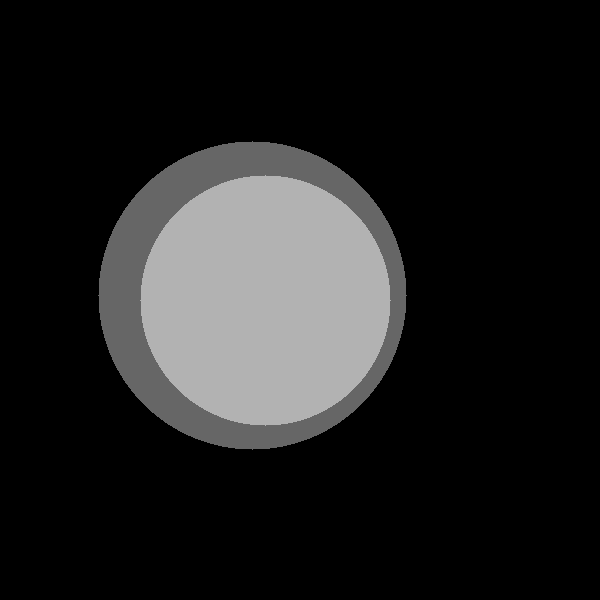
\includegraphics[width=3cm]{Images/Results/Results/drishti02/overlay.png} &
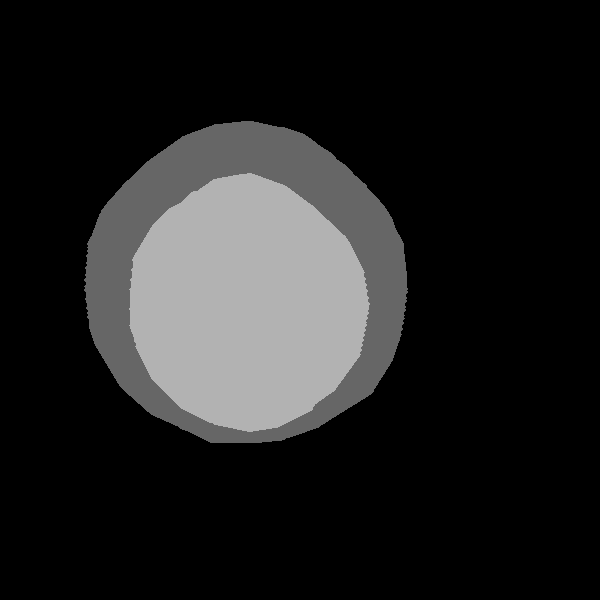
\includegraphics[width=3cm]{Images/Results/Results/drishti02/overlay_gt.png} \\

{} & {} & {} & CDR = 0.71 & CDR = 0.67 \\
{} & {} & {} & $\updownarrow$ & $\updownarrow$ \\
{} & {} & {} & Glaucomatous & Glaucomatous \\

\hline
\end{tabular}

\caption{\label{results}Qualitative results of the applied approach for glaucoma screening and diagnosis: (a) original retinal image, with OD location point (b) ROI extraction: sub-image around the OD, (c) k-means clustering (K=4), (d) joint OC-OD segmentation with CDR result and final diagnosis, (e) ground-truth joint OC-OD segmentation with CDR result and final diagnosis.}
\end{figure}
